\chapter {Postoje li osetljivi delovi
u ljudskom genomu?}
\setbookcodestyle

\section{Transformacija čoveka u miša}

\vspace{0.5cm}

\noindent \textbf{Koji blokovi genoma su slični i kako da ih
nađemo?}\\

\noindent \textbf{Kakav bi bio evolucioni scenario za
transformisanje jednog genoma u drugi?}\\

\begin{figure}[h!]
%\centering
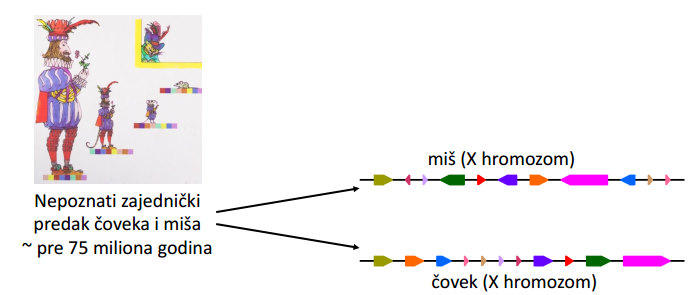
\includegraphics[scale=0.7]{poglavlja/6/slike/predak_X.PNG}
\caption{X hromozom miša i čoveka}
\label{slika:X}
\end{figure}

Kada je Šarl Pero opisao transformaciju čoveka u miša u delu "Mačak u čizmama", jedva je mogao očekivati da će 3 veka kasnije istraživanje pokazati da su ljudski i mišiji genom iznenađujuće slični.\\

Zapravo, ako bismo isekli 23 ljudska hromozoma na 280 delova i pomerali ove fragmente DNK, a zatim zalepili delove zajedno u novom redosledu, formiralo bi se 20 mišijih hromozoma. Međutim, evolucija nije koristila samo operaciju \textit{"cut and-paste"}, već manju promenu poznatu kao \textbf{preuređenje genoma}, što će biti naš  fokus u ovom poglavlju.\\

\newpage

\hspace{4cm}\large{\textbf{Blokovi sintenije}}\\

\begin{figure}[h!]
\centering
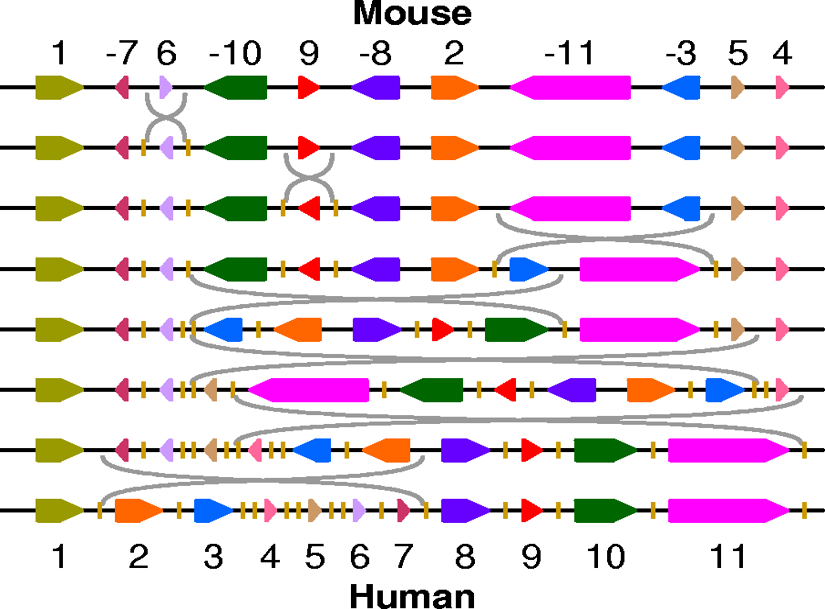
\includegraphics[scale=0.7]{poglavlja/6/slike/transformacija.png}
\caption{Blokovi sintenije}
\label{slika:X}
\end{figure}


\begin{figure}[h!]
\centering
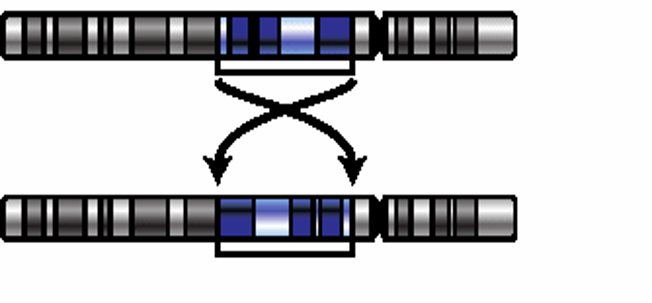
\includegraphics[scale=0.7]{poglavlja/6/slike/transformacijaa.png}
\caption{Blokovi sintenije}
\label{slika:X}
\end{figure}

Svaki od jedanaest obojenih segmenata na slici predstavlja blok sličnih gena i naziva se \textbf{blok sintenije}. U nastavku će biti objašnjeno kako se izgrađuju blokovi sintenije i šta označavaju levi i desni pravac blokova.\\

Slika 6.2 prikazuje niz 7 promena koje transformišu mišiji X hromozom u ljudski X hromozom. Nažalost, ovaj niz od 7 promena predstavlja samo jedan od 1.070 različitih scenarija od 7 promena koji transformišu X hromozom miša u X hromozom čoveka.\\

\noindent \textbf{Možemo  li pretvoriti X hromozom miša u ljudski X hromozom koristeći samo šest promena}?\\

Bez obzira na to koliko promena razdvaja mišije i ljudske X hromozome, promene moraju biti \textit{retki genomski događaji}. Zapravo, obično preuređeni genomi uzrokuju smrt ili sterilnost mutiranog organizma, čime se sprečava prenošenje preuređenja na narednu generaciju. Međutim, mali deo preuređenja genoma moze imati pozitivan efekat na preživljavanje i propagirati se kroz vrstu kao rezultat prirodne selekcije. Kada stanovništvo postane izolovano od ostatka njene vrste dovoljno dugo, preuređenja mogu čak stvoriti i novu vrstu.\\

Promenu mozemo zamisliti kao prekid genoma sa obe strane hromozomskog intervala, pomeranje intervala, a zatim lepljenje rezultujućih segmenata u novom redosledu.\\

\begin{figure}[h!]
\centering
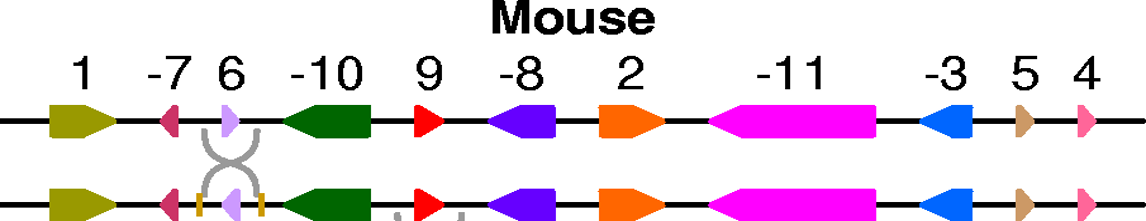
\includegraphics[scale=0.32]{poglavlja/6/slike/niz1.png}
\caption{Promena 1}
\label{slika:X}
\end{figure}

\begin{figure}[h!]
\centering
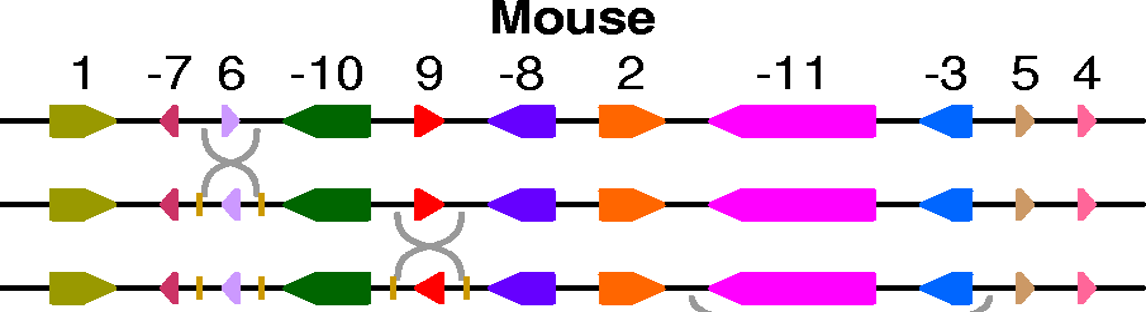
\includegraphics[scale=0.32]{poglavlja/6/slike/niz2.png}
\caption{Promena 2}
\label{slika:X}
\end{figure}

\begin{figure}[h!]
\centering
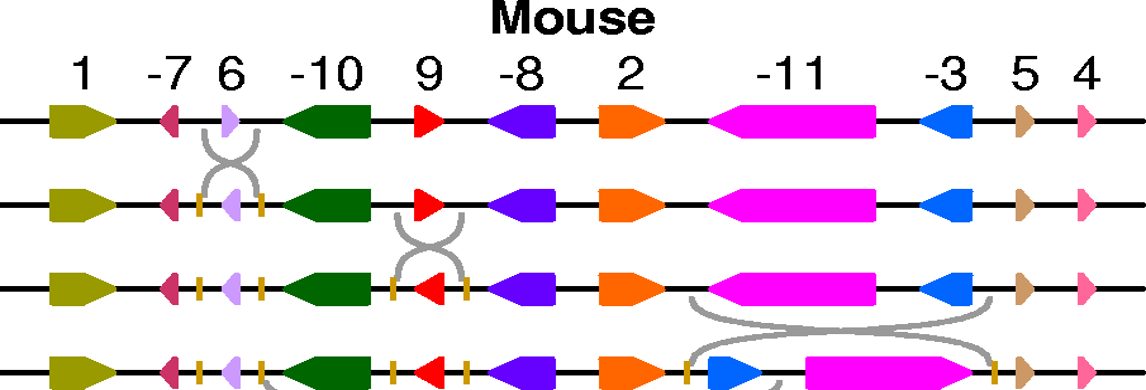
\includegraphics[scale=0.32]{poglavlja/6/slike/niz3.png}
\caption{Promena 3}
\label{slika:X}
\end{figure}

\begin{figure}[h!]
\centering
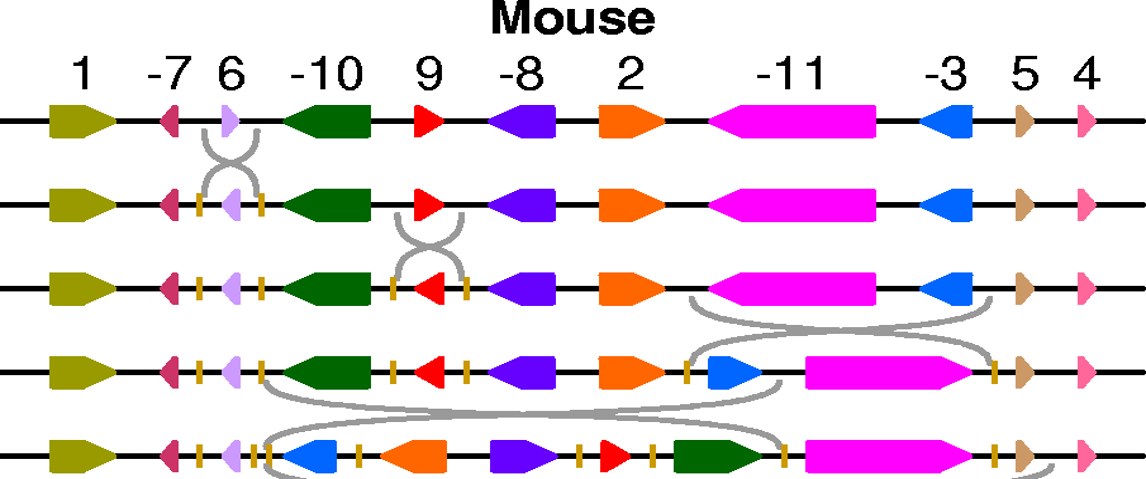
\includegraphics[scale=0.32]{poglavlja/6/slike/niz4.png}
\caption{Promena 4}
\label{slika:X}
\end{figure}

\begin{figure}[h!]
\centering
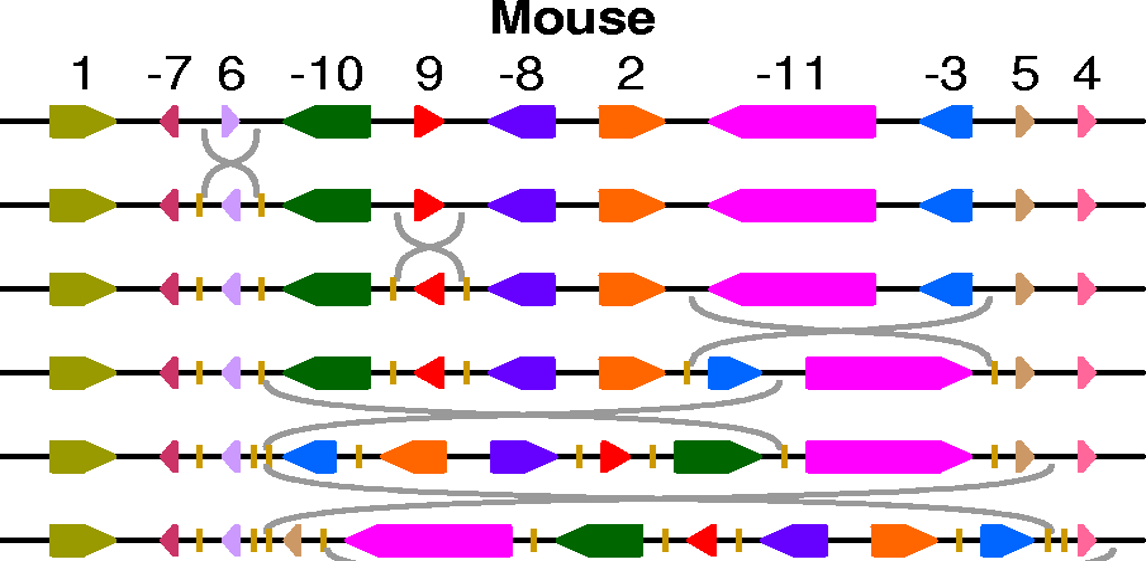
\includegraphics[scale=0.32]{poglavlja/6/slike/niz5.png}
\caption{Promena 5}
\label{slika:X}
\end{figure}

\begin{figure}[h!]
\centering
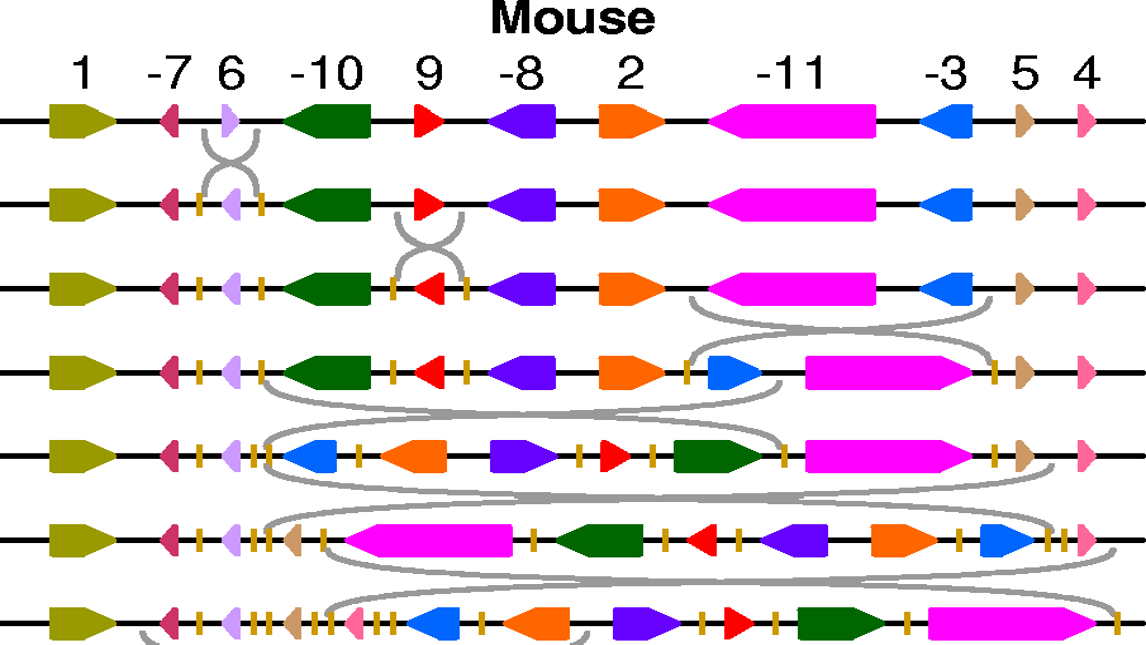
\includegraphics[scale=0.32]{poglavlja/6/slike/niz6.png}
\caption{Promena 6}
\label{slika:X}
\end{figure}

\begin{figure}[h!]
\centering
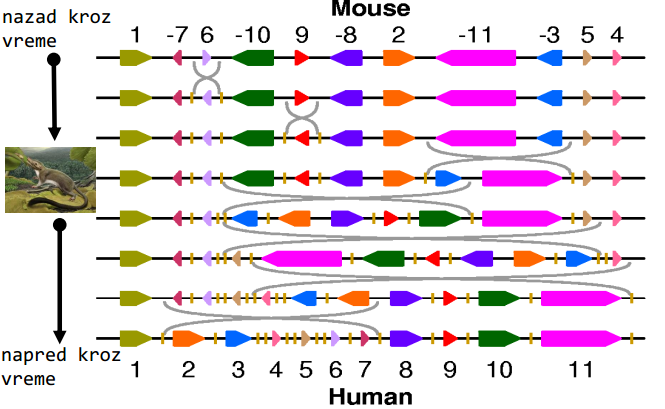
\includegraphics[scale=0.32]{poglavlja/6/slike/niz7.png}
\caption{Završena transformacija}
\end{figure}

\newpage
Slika 6.10 predstavlja transformaciju mišijeg X hromozoma u ljudski X hromozom sa sedam promena. Svaki sinteni blok je jedinstveno obojen i označen celim brojem između 1 i 11. Pozitivni ili negativni znak svakog celog broja ukazuje na smer sintenog bloka (pokazivanje desno ili levo, respektivno). Dva kratka vertikalna segmenta obeležavaju krajnje tačke obrnutog intervala u svakom preokretu.\\

Pretpostavimo da je evolucijski scenario tačan i recimo peti sinteni blok od vrha predstavlja uređenje hromozoma pretka. Zatim su se desile prve četiri promene na evolucionom putu od miša do zajedničkog pretka, a poslednje tri promene su se desile na evolucionom putu od zajedničkog pretka ka coveku.

\newpage
\section{Sortiranje po promenama}

\hspace{0.7cm} Glavni problem je, kao sto je pomenuto u uvodu, nalaženje minimalnog broja promena koje omogućavaju transformaciju X hromozona miša u X hromozom čoveka.\\

\noindent Možemo posmatrati niz blokova sintenije numerisanih kao na slici 6.11.\\

\begin{figure}[h!]
\centering
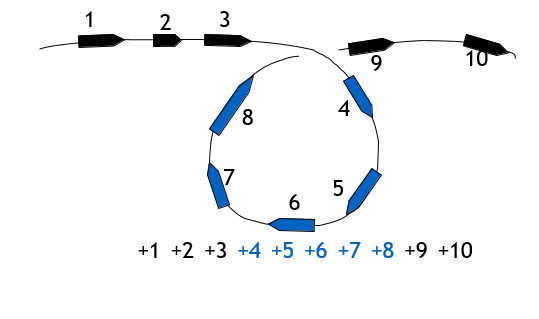
\includegraphics[scale=0.5]{poglavlja/6/slike/promene1.PNG}
\caption{Blokovi sintenije}
\label{slika:X}
\end{figure}

\begin{figure}[h!]
\centering
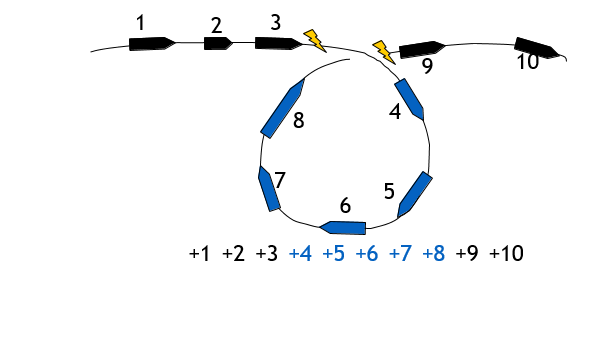
\includegraphics[scale=0.5]{poglavlja/6/slike/promene2.PNG}
\caption{}
\label{slika:X}
\end{figure}

\begin{figure}[h!]
\centering
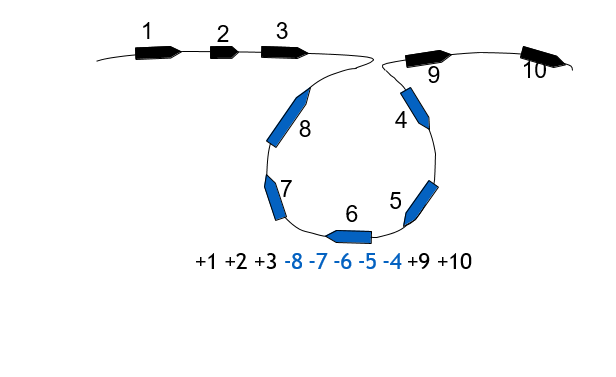
\includegraphics[scale=0.5]{poglavlja/6/slike/promene3.PNG}
\caption{}
\label{slika:X}
\end{figure}

\noindent Nakon izvršene promene, dobijamo preuređen niz blokova sintenije u genomu.\\

\begin{figure}[h!]
\centering
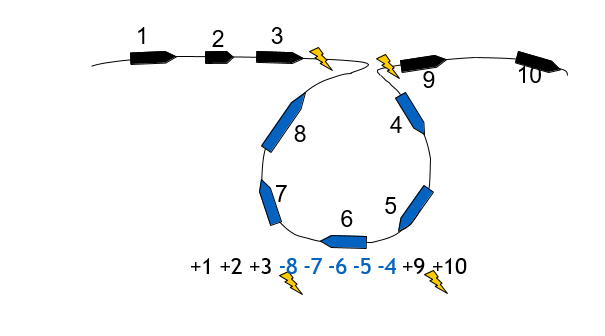
\includegraphics[scale=0.5]{poglavlja/6/slike/promene4.PNG}
\caption{2 tačke prekida}
\label{slika:X}
\end{figure}

\noindent Promene u genomu su dovele do stvaranja dve tačke prekida koje predstavljaju poremećaj u redosledu gena u genomu (Slika 14).\\

\noindent Posmatraćemo 2 scenarija sa različitim brojem promena.\\

\begin{figure}[h!]
\centering
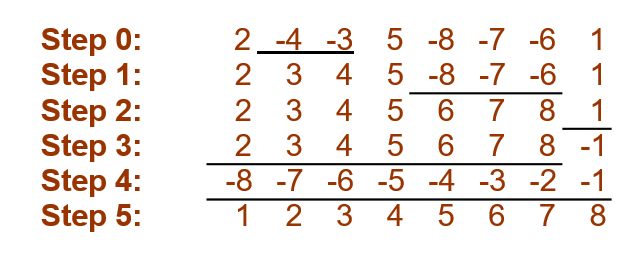
\includegraphics[scale=0.6]{poglavlja/6/slike/scenario5.PNG}
\caption{Scenario sa 5 promena}
\label{slika:X}
\end{figure}

\begin{figure}[h!]
\centering
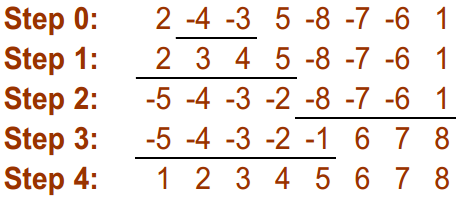
\includegraphics[scale=0.7]{poglavlja/6/slike/scenario4.PNG}
\caption{Scenario sa 4 promene}
\label{slika:X}
\end{figure}

\begin{definicija}{\textbf{Rastojanje premutacija} je najmanji broj promena potrebnih za transformisanje jedne premutacije u drugu.}
\end{definicija}

\noindent Naredni problem koji posmatramo je \textbf{problem sortiranja po promenama} koji predstavlja izračunavanje rastojanja između date permutacije i identične permutacije (+1 +2 ... +n)

\textbf{Ulaz}: permutacija P\\
\indent \textbf{Izlaz}: rastojanje između permutacije P i identične permutacije\\

\vspace{1cm}

\hspace{2cm} \textbf{Pohlepno sortiranje po promenama}\\

Prva aproksimacija rastojanja između 2 permutacije je \textbf{pohlepno sortiranje po promenama}.\\

\begin{figure}[h!]
\centering
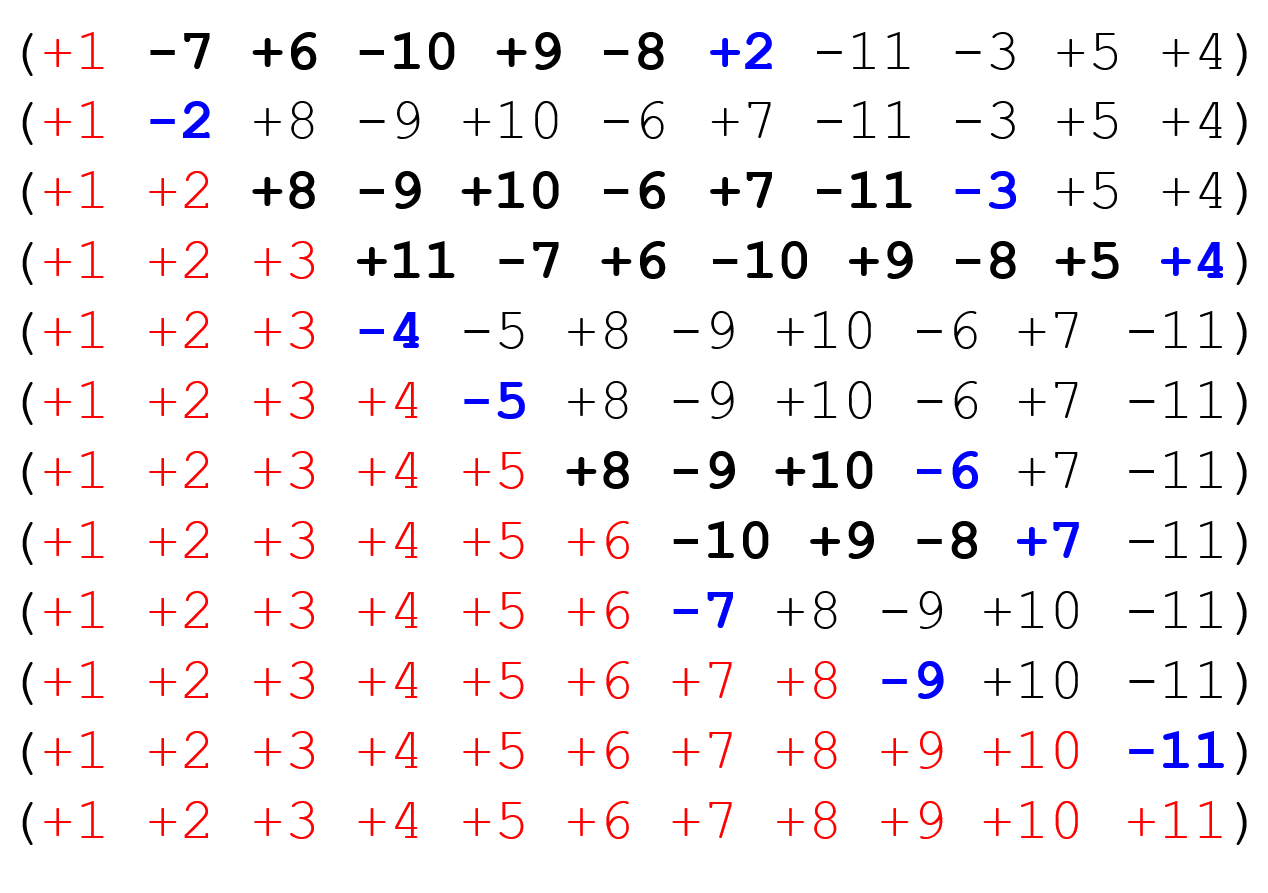
\includegraphics[scale=0.4]{poglavlja/6/slike/greedy_sort.png}
\caption{Pohlepno sortiranje}
\label{slika:X}
\end{figure}

Prvi korak je da se izvrši promena koji postavlja +1 na pravo mesto (na prvu poziciju), a zatim slede promene koji postavljaju
+2 na drugu poziciju, i tako dalje. Na primer, element 1 je već na pravom mestu i ima ispravan znak (+) u X hromozomu miša, ali element 2 nije na ispravnom položaju. Element 1 možemo zadržati fiksiran i premestiti element 2 na pravi položaj jednom promenom. Još jedna promena je potrebna da bi element 2 imao ispravan znak.\\

\noindent Daljim iteriranjem postupka dovodimo sve veće elemente na njihove ispravne pozicije.

\newpage
\begin{definicija}{Element k u permutaciji P = $(p_1, p_2, ..., p_n$) je \textbf{sortiran}, ako je $p_k = k$, a u suprotnom je \textbf{nesortiran}.}
\end{definicija}

\begin{definicija}{Permutacija P je \textbf{k-sortirana}, ako je prvih k-1 elemenata sortirano, a k-ti element nesortiran.}
\end{definicija}

\noindent Sledeći primer pokazuje da je pohlepno sortiranje loša aproksimacija rastojanja između dve permutacije.\\

\begin{figure}[h]
\centering
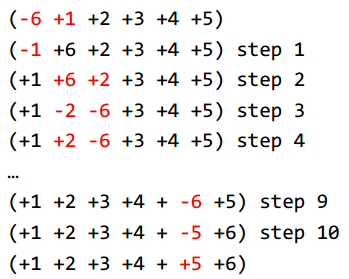
\includegraphics[scale=0.75]{poglavlja/6/slike/los_greedy.PNG}
\caption{Pohlepno sortiranje}
\label{slika:X}
\end{figure}

\begin{figure}[h]
\centering
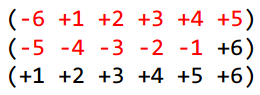
\includegraphics[scale=0.75]{poglavlja/6/slike/kraci.PNG}
\caption{Kraći način}
\label{slika:X}
\end{figure}

\section{Teorema o prekidnoj tački}

\hspace{0.7cm}Uočimo da su uzastopni elementi (npr. (+12 +13)) poželjni, jer se javljaju u istom redosledu kao i u identičnoj permutaciji. Takodje, i (-11 -10) su poželjni, jer se mogu inverzijom postaviti u pravi redosled. Ova dva para elemenata imaju zajedničku osobinu da je drugi element za 1 veci od prvog. Stoga, definišemo pojam suseda.

\begin{definicija}{$(p_i, p_{i+1})$ u permutaciji $P = (p_1, p_2, ..., p_n)$ predstavljaju \textbf{susede}, ako je $p_{i+1} - p_i = 1$, a u suprotnom čine \textbf{prekid}.}
\end{definicija}

\begin{figure}[h!]
\centering
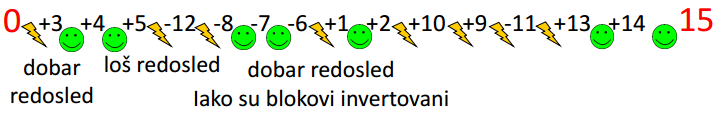
\includegraphics[scale=0.75]{poglavlja/6/slike/dobar_los.PNG}
\caption{Susedi i prekidi}
\label{slika:X}
\end{figure}

Važi:\\
$$ adjacencies(P) + breakpoints(P) = |P| + 1.$$

\hspace{1cm}

\large{\textbf{Sortiranje po promenama eliminacijom prekidnih tacaka}}\\

\begin{figure}[h]
\centering
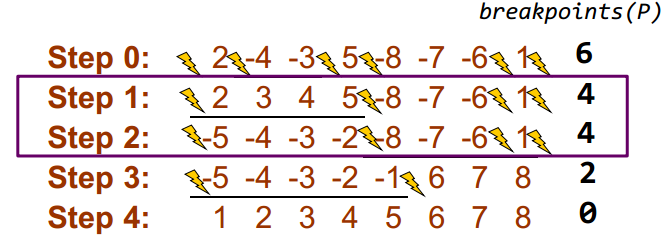
\includegraphics[scale=0.7]{poglavlja/6/slike/koliko.PNG}
\caption{}
\label{slika:X}
\end{figure}

\noindent Koliko prekidnih tačaka može biti eliminisano u jednoj promeni?\\

\vspace{1cm}
\hspace{2.3cm}\textbf{Teorema o prekidnoj tački}\\

\hspace{0.5cm} rastojanje između permutacija $\geq$ breakpoints(P)/2\\

\begin{itemize}
\item{Nema garancije da će svaka promena eliminisati 2 prekidne tačke (step 2)}

\item{Najveći broj promena bi bio za permutaciju (+n +(n - 1) ... +1) i iznosi n+1 (gornja granica)}

\item{Donja granica: (n + 1)/2}
\end{itemize}

\noindent Velika razlika između donje i gornje granice nam sugeriše da moramo preći na drugi način za rešavanje ovog problema.
\newpage
\section{Preuređivanje u multihromozomalnim genomima}

Umesto što posmatramo preuređivanje gena u okviru
jednog hromozoma (hromozom X kod čoveka i miša),
generalizujemo problem i posmatramo sve genome
hromozoma.\\

U ovoj generalizaciji će biti više oblika
preuređivanja blokova u genomu (do sada su bila
samo obrtanja).\\

Problem je naizgled komplikovaniji, u nastavku će
se ispostaviti da nije tako.\\

\subsection{Translokacije, fuzije i fizije}

\begin{figure}[h!]
\centering
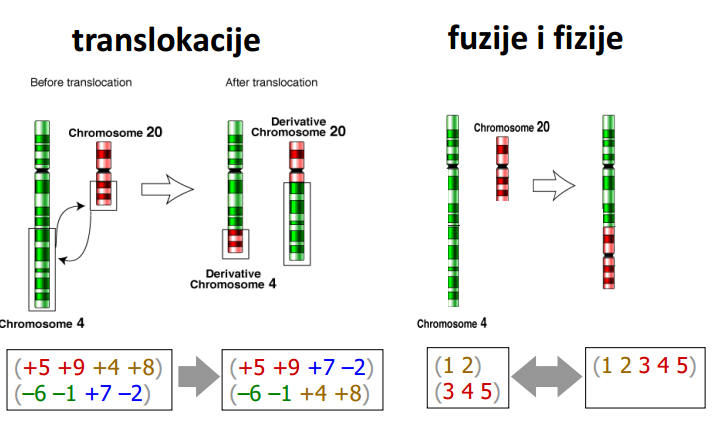
\includegraphics[scale=0.45]{poglavlja/6/slike/preuredjivanja.PNG}
\caption{Translokacije, fuzije i fizije}
\label{slika:X}
\end{figure}

Za modeliranje translokacija posmatramo multihromozomalni genom sa k hromozoma
kao permutaciju koja je podeljena na k delova.\\

Na primer, genom
(+1 +2 +3 +4 +5 +6) (+7 +8 +9 +10 +11) je sastavljen od dva hromozoma (+1
+2 +3 +4 +5 +6) i (+7 +8 +9 +10 +11). \\

Translokacija razmenjuje segmente
različitih hromozoma, npr, translokacija dva hromozoma
(+ 1 + 2 + 3 + 4 + 5 + 6) (+ 7 + 8 + 9 +10 +11)
može dovesti do sledeća 2 hromozoma
(+ 1 + 2 + 3 + 4 + 9 +10 +11) (+ 7 + 8 + 5 + 6 ).
Možemo zamišljati translokaciju kao prvo cepanje svakog od hromozoma
( + 1 + 2 + 3 + 4 + 5 + 6 ) ( + 7 + 8 + 9 + 1 0 + 1 1 )
na 2 dela,
( + 1 + 2 + 3 + 4 ) (+ 5 + 6 ) (+ 7 + 8 ) (+ 9 + 1 0 + 1 1 ) ,
a zatim lepljenje rezultujućih segmenata u 2 nova hromozoma,
(+ 1 + 2 + 3 + 4 + 9 +10 +11) (+ 7 + 8 + 5 + 6 ) .\\

Preuređenja u multihromozomalnim genomima nisu ograničena na promene i translokacije. Ona takođe uključuju hromozomske fuzije, koje spajaju 2 hromozoma u 1, kao i fisije, koje dele 1 hromozom na 2 hromozoma.\\

Na primer, 2 hromozoma
( + 1 + 2 + 3 + 4 + 5 + 6 ) ( + 7 + 8 + 9 + 1 0 + 1 1 ) mogu biti fuzionisani (spojeni) u 1 hromozom (+ 1 + 2 + 3 + 4 + 5 + 6 + 7 + 8 + 9 +10 + 1 1 ).
Sledeća fisija ovog hromozoma moze dovesti do 2 hromozoma ( + 1 + 2 + 3 + 4 ) (+5+6+7+8+9+10+11).\\

Pre pet miliona godina, ubrzo nakon razdvajanja čoveka i šimpanze, fuzija
dva hromozoma (nazvana 2A i 2B) u jednom od naših predaka stvorila je ljudski hromozom 2 i smanjila broj hromozoma sa 24 na 23.

%\newpage
\section{Problem rastojanja 2-prekida}

\subsection{Od linearnih do cirkularnih hromozoma}

\indent Sada se fokusiramo na jedan od hromozoma u multihromozomalnom genomu i razmotrimo transformacije promene kružnog hromozoma P = (+ a -b -c + d) u Q = (+ a -b
-d + c). \\

\noindent Uvodimo pojam crnih usmerenih i crvenih neusmerenih grana.

\begin{figure}[h!]
\centering
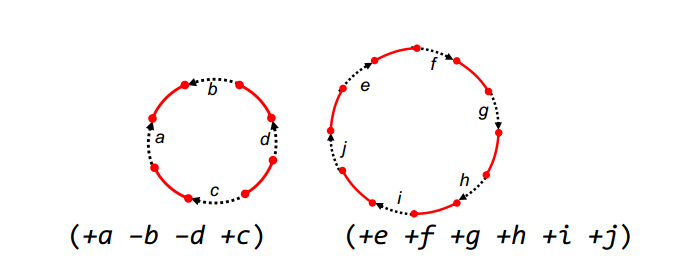
\includegraphics[scale=0.6]{poglavlja/6/slike/crne_crvene.PNG}
\caption{Hromozomi P i Q}
\label{slika:X}
\end{figure}

\noindent \textbf{Crne usmerene grane} predstavljaju blokove sintenije.

\noindent \textbf{Crvene neusmerene grane} povezuju susedne blokove sintenije.\\

Možemo nacrtati Q na različite načine, zavisno od toga kako se odlučimo da uredimo crne grane. Slika 6.24 prikazuje dve takve ekvivalentne reprezentacije.\\

\begin{figure}[h!]
\centering
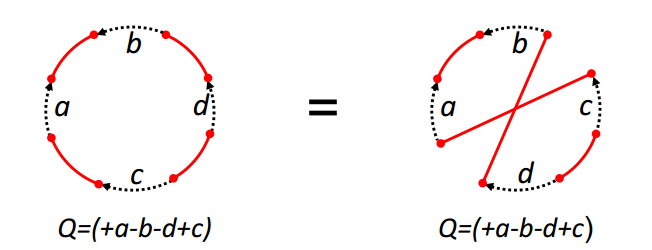
\includegraphics[scale=0.5]{poglavlja/6/slike/ekvivalentne.PNG}
\caption{Ekvivalentne reprezentacije hromozoma Q}
\label{slika:X}
\end{figure}

\newpage
Iako je prvi crtež Q na slici njegova najprirodnija reprezentacija, koristićemo drugu reprezentaciju, jer su joj crne grane raspoređene kružno u potpuno istom redosledu kako se pojavljuju u prirodnoj reprezentaciji P = (+a -b -c +d).\\

Kao što je prikazano na slici 6.25, fiksiranje crnih grana omogućava nam da vizualizujemo efekat promena. Kao sto možemo videti, promena briše ("deli") dve crvene grane iz P (povezivanje $b$ sa $c$ i $d$ sa $a$) i zamenjuje ih sa dve nove crvene grane (povezivanje $b$ sa $d$ i $c$ sa $a$). Ova promena se naziva \textbf{obrtanje}.\\

\begin{figure}[h!]
\centering
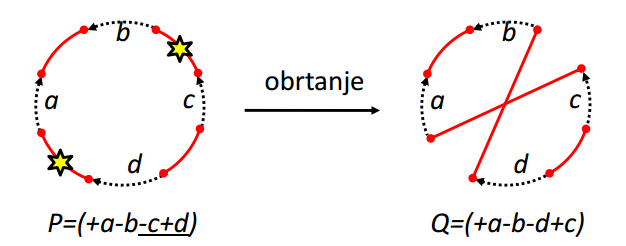
\includegraphics[scale=0.6]{poglavlja/6/slike/obrtanje.PNG}
\caption{Obrtanje}
\label{slika:X}
\end{figure}

Slika 6.26 ilustruje fiziju P = (+ a -b -c + d) u Q = (+ a -b) (- c + d).
Inverzna operacija fiziji odgovara fuziji dva hromozoma iz Q u hromozom P. Operacije fuzije i fizije, kao i promene, odgovaraju brisanju dve grane u jednom genomu i njihovim zamenjivanjem sa 2 nove grane u drugom genomu.\\

\begin{figure}[h!]
\centering
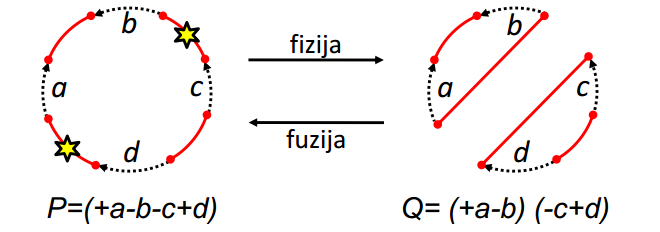
\includegraphics[scale=0.6]{poglavlja/6/slike/fizija_fusija.PNG}
\caption{Fizija i fuzija}
\label{slika:X}
\end{figure}

\newpage
Translokacija koja uključuje dva linearna hromozoma takođe se može simulirati cirkularizacijom ovih hromozoma, a zatim zamenjivanjem dve crvene grane sa dve različite crvene grane, kao što je prikazano na slici 6.27. Zbog toga se mogu objediniti ova 4 različita tipa preuređenja. Svi oni se mogu posmatrati kao cepanje 2 crvene grane grafa genoma i zamena sa dve nove crvene grane na ista 4 cvora. \\
Iz tog razloga definišemo opštu operaciju na grafu genoma
koja zamenjuje crvenu granu sa dve nove crvene grane pri čemu čvorovi ostaju isti i nazivamo je \textbf{2-prekid}.\\

\begin{figure}[h]
\centering
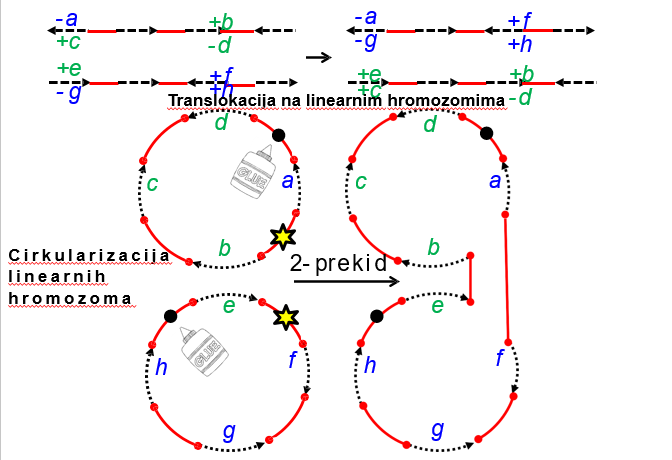
\includegraphics[scale=0.6]{poglavlja/6/slike/2_prekid_1.PNG}
\caption{2-prekid}
\label{slika:X}
\end{figure}

\newpage
\begin{figure}[h]
\centering
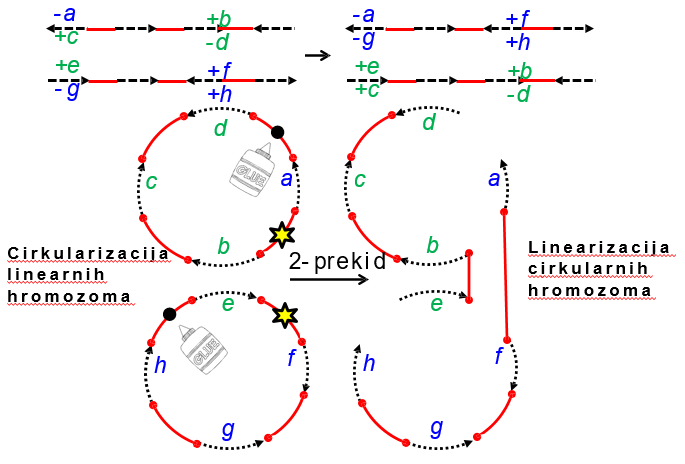
\includegraphics[scale=0.6]{poglavlja/6/slike/2_prekid_2.PNG}
\caption{Objedivanje sva 4 preuredjenja}
\label{slika:X}
\end{figure}

\subsection{Rastojanje 2-prekida}

\begin{definicija} {Rastojanje 2-prekida d(P,Q): Minimalni broj 2-prekida koji transformišu genom P u genom Q.}
\end{definicija}
\begin{definicija} {Problem rastojanja 2-prekida: Naći rastojanje 2-prekida između dva genoma.}
\end{definicija}

\textbf{Ulaz}. Dva genoma nad istim skupom blokova
sintenije. \\

\textbf{Izlaz}. Rastojanje 2-prekida između ovih genoma.\\

\newpage
\section{Grafovi prekidnih tačaka}
\indent Za izračunavanje rastojanja 2-prekida konstruisaćemo graf za upoređivanje dva genoma.\\

Posmatrajmo genome {\color{red}P} i {\color{blue}Q}.

\begin{figure}[h!]
\minipage{0.45\textwidth}
  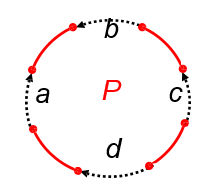
\includegraphics[width=\linewidth]{poglavlja/6/slike/P.PNG}
  \caption{Slika 29: Genom P}
\endminipage\hfill
\minipage{0.42\textwidth}
  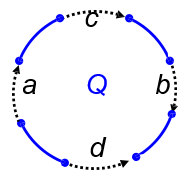
\includegraphics[width=\linewidth]{poglavlja/6/slike/Q.PNG}
  \caption{Genom Q}
\endminipage\hfill
\end{figure}

Genom {\color{blue}Q} mozemo predstaviti i na drugi nacin.
\begin{figure}[h!]
\centering
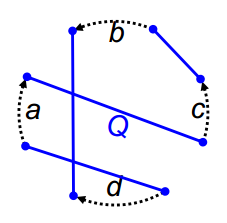
\includegraphics[scale=0.75]{poglavlja/6/slike/Q2.PNG}
\caption{Drugačija reprezentacija genoma Q}
\label{slika:X}
\end{figure}

\newpage
\noindent Nadgradnjom genoma {\color{red}P} i {\color{blue}Q} dobijamo $BreakpointGraph({\color{red}P}, {\color{blue}Q}).$
\begin{figure}[h]
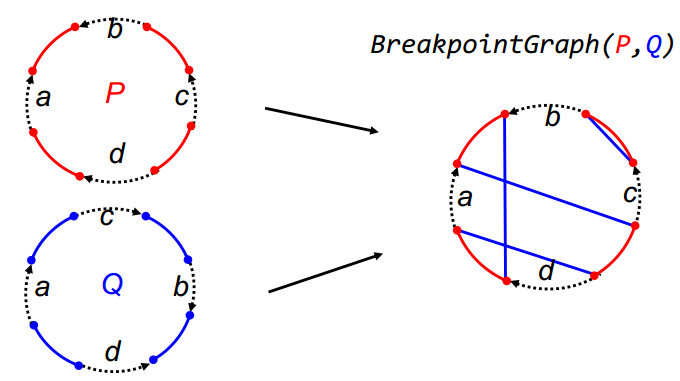
\includegraphics[scale=0.7]{poglavlja/6/slike/breakpointgraph.PNG}
\caption{Nadgradnja genoma P i Q}
\label{slika:X}
\end{figure}

{\color{red} Crvene} i crne grane u grafu prekidnih tačaka formiraju genom P.\\

{\color{blue} Plave} i crne grane u grafu prekidnih tačaka  formiraju genom Q.\\

{\color{red} Crvene} i {\color{blue} plave} grane formiraju \textbf{alternirajuće crveno-plave cikluse}.
\begin{figure}[h!]
\centering
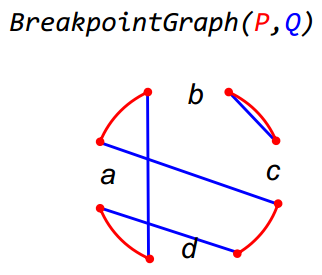
\includegraphics[scale=0.7]{poglavlja/6/slike/alternirajuci.PNG}
\caption{Alternirajući crveno-plavi ciklusi }
\label{slika:X}
\end{figure}

\newpage
\noindent Koristimo oznaku \textbf{cycle(P, Q)}: broj alternirajućih crveno-plavih ciklusa.\\

\noindent Šta predstavlja cycle(P, Q)?
\begin{figure}[h!]
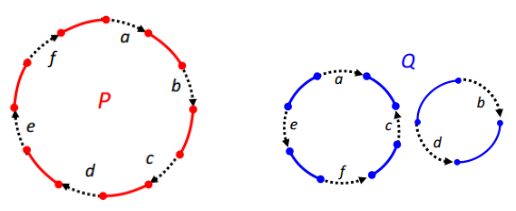
\includegraphics[scale=0.7]{poglavlja/6/slike/PiQ1.PNG}
\caption{Grafovi genoma P i Q}
\label{slika:X}
\end{figure}

\begin{enumerate}
\item {korak: Poređamo crne grane genoma Q u isti redosled kao u genomu P}
\item {korak: Nadgradnja genoma P i Q u jedan}
\item {korak: Uklanjanje crnih grana}
\end{enumerate}

\begin{figure}[h!]
\centering
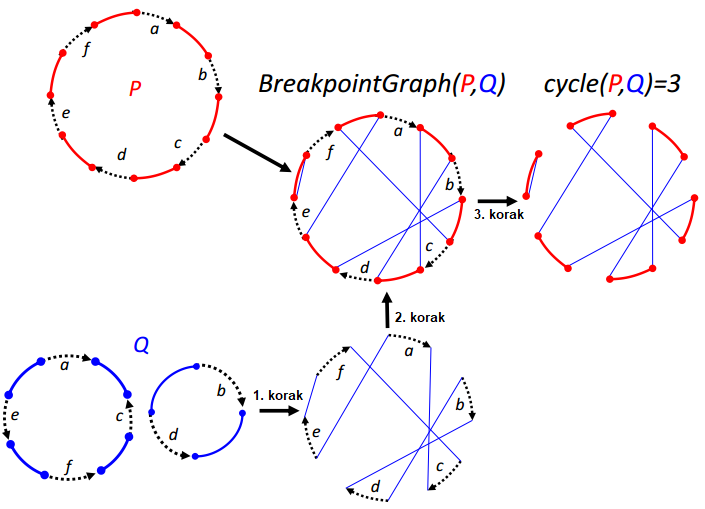
\includegraphics[scale=0.55]{poglavlja/6/slike/cycle.PNG}
\caption{cycle(P,Q)}
\label{slika:X}
\end{figure}
\newpage
\noindent \textbf{ Za dato P, koje Q maksimizuje cycle(P, Q)?}\\

\begin{figure}[h!]
\centering
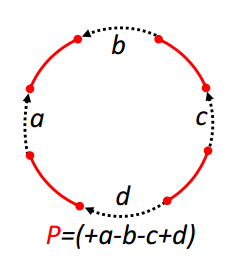
\includegraphics[scale=0.7]{poglavlja/6/slike/Pabcd.PNG}
\caption{Genom P}
\label{slika:X}
\end{figure}

U slučaju da P i Q imaju isti broj blokova sintenije, označimo taj broj sa \textbf{Blocks(P, Q)}. Ako su P i Q identični, njihov graf prekidnih tačaka se sastoji od Blocks(P, Q) ciklusa dužine 2 od kojih svaki sadrži jednu crvenu i jednu plavu granu. Cikluse dužine 2 nazivamo \textbf{identičkim ciklusima}, a graf prekidnih tačaka formiran na osnovu identičkih genoma nazivamo \textbf{identičkim grafom prekidnih tačaka}.

\begin{figure}[h!]
\centering
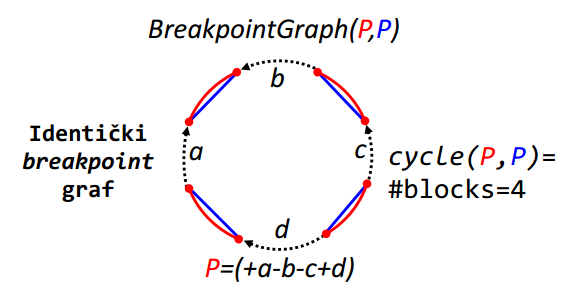
\includegraphics[scale=0.6]{poglavlja/6/slike/identicki.PNG}
\caption{Identički graf prekidnih tačaka}
\label{slika:X}
\end{figure}
\newpage
Preuređenje genoma utiče na crveno-plave cikluse.\\

Svaka transformacija $P\rightarrow Q$ odgovara transformaciji:

\begin{figure}[h!]
\centering
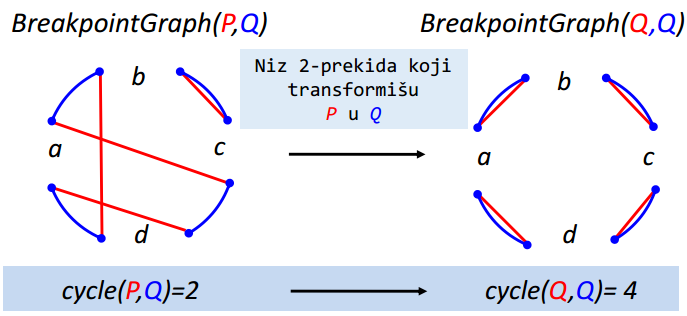
\includegraphics[scale=0.7]{poglavlja/6/slike/transfBreakpoint.PNG}
\caption{Trasnformacija $P\rightarrow Q$ }
\label{slika:X}
\end{figure}

%newline
 Preuređenja genoma takođe utiču i na cycle(P, Q):

\begin{figure}[h!]
\centering
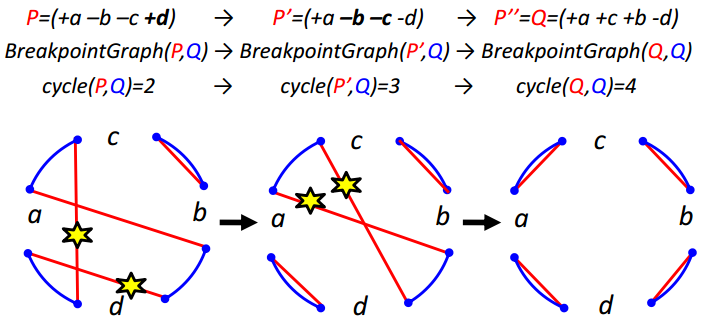
\includegraphics[scale=0.7]{poglavlja/6/slike/preuredjenja_cycle.PNG}
\caption{Slika 39: Uticaj preuređenja na cycle(P,Q)}
\label{slika:X}
\end{figure}

\newpage
\section{Teorema o rastojanju 2-prekida}
Posmatramo problem sortiranja po 2-prekidima:
\begin{figure}[h!]
\centering
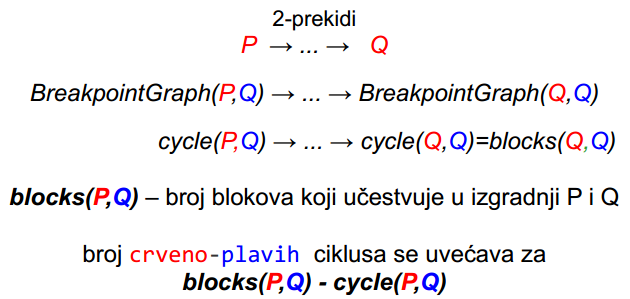
\includegraphics[scale=0.7]{poglavlja/6/slike/sortiranje2prekidi.PNG}
\caption{Sortiranje po 2-prekidima}
\label{slika:X}
\end{figure}

\noindent \textbf{Koliko može svaki 2-prekid da doprinese ovom uvećanju?}\\

\noindent 2-prekid može izmeniti cycle(P, Q) za 1.\\

\begin{figure}[h!]
\centering
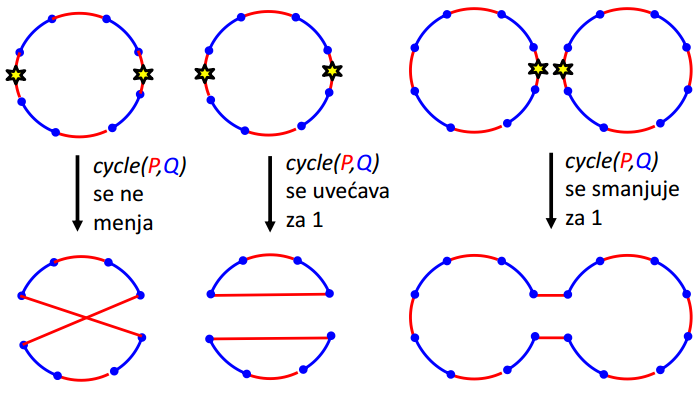
\includegraphics[scale=0.5]{poglavlja/6/slike/izmena2prekidima.PNG}
\caption{}
\label{slika:X}
\end{figure}
\newpage
\noindent \textbf{Postoji 2-prekid povecanje velicine cycle(P, Q) za 1}
\begin{figure}[h]
\centering
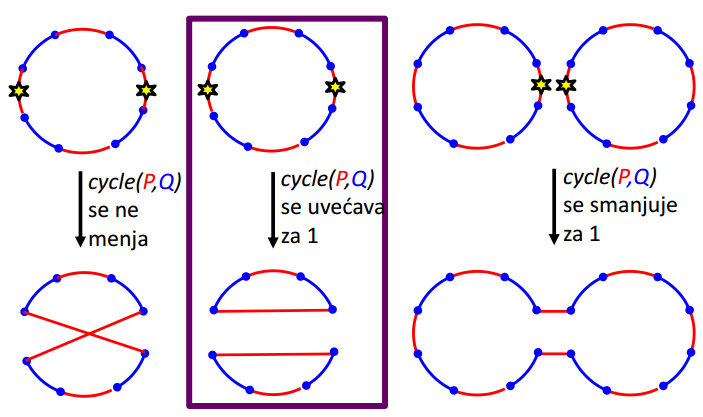
\includegraphics[scale=0.6]{poglavlja/6/slike/izmena2prekidima2.PNG}
\caption{}
\label{slika:X}
\end{figure}

\noindent \textbf{Teorema o rastojanju 2-prekida}
\begin{itemize}
    \item Svaki 2-prekid povećava broj ciklusa najviše za 1
    \item Za svaki 2-prekid postoji povećanje broja ciklusa za tačno 1
    \item Svako sortiranje po 2-prekidima mora povećati broj ciklusa za $blocks(P,Q) - cycle(P, Q)$
    \item 2-prekid rastojanje između genoma P i Q:   $$d(P,Q) = blocks(P, Q) - cycle(P,Q)$$
\end{itemize}

\noindent \textbf{Rastojanje 2-prekida između genoma čoveka i miša}
\begin{itemize}
    \item Genomi čoveka i miša se mogu rastaviti na 280 blokova sintenije (dužine bar pola miliona nukleotida)
    \item Graf prekidnih tačaka nad ovim blokovima ima ukupno 35 ciklusa
    \item Na osnovu teoreme o rastojanju 2-prekida:
    $$d(H, M) = blocks(H, M) - cycle(H, M) = 280 - 35 = 245$$
    \item Postoje različite verzije scenarija sa 245 koraka.
    \item Pravi evolutivni scenario je možda imao i više od 245 koraka.
\end{itemize}
\newpage
\hspace{3cm} {\textbf{Shortest rearrangement scenario}}

\begin{figure}[h!]
\centering
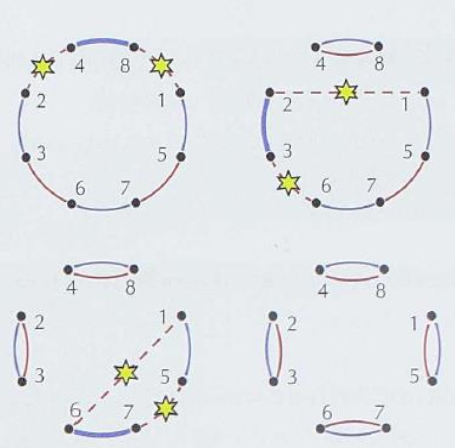
\includegraphics[scale=0.65]{poglavlja/6/slike/izmena2prekidima3.PNG}
\caption{Shortest rearrangement scenario}
\label{slika:X}
\end{figure}

%\newpage
\noindent $\textbf{ShortestRearrangementScenario(P, Q)}$\\
\indent \textbf{output P}\\
\indent $RedEdges \leftarrow ColoredEdges(P)$\\
\indent $BlueEdges \leftarrow ColoredEdges(Q)$\\
\indent $BreakpointGraph \leftarrow$ the graph formed by $RedEdges$ and $BlueEdges$\\
\indent \textbf{while} \hspace{0.2cm} $BreakpointGraph$ has a non-trivial cycle Cycle\\
\indent \indent $(j, i') \leftarrow$ an arbitary edge from $BlueEdges$ in a nontrivial red \\
\indent \indent blue cycle\\
\indent \indent $(i, j) \leftarrow$ an edge from $RedEdges$ originating  at node $j$\\
\indent \indent $(i', j') \leftarrow$ an edge from $RedEdges$ originating at node $i'$\\
\indent \indent $RedEdges \leftarrow RedEdges$ with edges $(i, j)$ and $(i', j')$ removed\\
\indent \indent $RedEdges \leftarrow$ RedEdges with edges $(j, i')$ and $(j', i)$ added\\
\indent \indent $BreakpointGraph \leftarrow$ the graph formed by $RedEdges$ and $BlueEgdes$\\
\indent \indent $P \leftarrow \textbf{2-BreakOnGenome(P, i, i', j, j')}$\\
\indent \indent \textbf{output P}\\

\noindent $2-BreakOnGenome(P, i, i', j, j')$ - uklanja grane $(i, i')$ i dodaje grane $(i, j)$ i $(i', j')$ (genom predstavljen grafom prekidnih tačaka)

\newpage

\section{Zadaci sa vezbi}

\setexamplecodestyle
\subsection{ChromosomeToCycle}
\lstinputlisting[language=Python]{poglavlja/6/kodovi/ChromosomeToCycle.py}

\subsection{CycleToChromosome}
\lstinputlisting[language=Python]{poglavlja/6/kodovi/CycleToChromosome.py}

\subsection{GreedySorting}
\lstinputlisting[language=Python]{poglavlja/6/kodovi/GreedySorting.py}

\subsection{ShortestRearrangementScenario}
\lstinputlisting[language=Python]{poglavlja/6/kodovi/ShortestRearrangementScenario.py}

